\documentclass[conference,10pt]{IEEEtran}
\IEEEoverridecommandlockouts
\usepackage[T1]{fontenc}
\usepackage{graphicx,booktabs,amsmath,amssymb,xcolor,url,xspace,textcomp}
\usepackage[hidelinks]{hyperref}
\hypersetup{pdftitle={reBot Cube Grasping: Staged RL in Simulation and Perception-IK Control on Hardware}, pdfauthor={Jeong Hwan Lee}}
\usepackage{array,tikz}
\usetikzlibrary{positioning,arrows.meta}
\def\UrlBreaks{\do\/\do\_\do\.\do\-}\def\UrlFont{\small\ttfamily}\newcommand{\code}[1]{\path{#1}}
\definecolor{simF}{HTML}{E3F2FD}\definecolor{simS}{HTML}{1E88E5}
\definecolor{hwF}{HTML}{FFEBEE}\definecolor{hwS}{HTML}{E53935}
\definecolor{okF}{HTML}{E8F5E9}\definecolor{okS}{HTML}{43A047}

\begin{document}
\title{reBot Cube Grasping:\\Staged RL in Simulation and\\Perception--IK Control on Hardware}
\author{\IEEEauthorblockN{Jeong Hwan Lee}
\IEEEauthorblockA{Technical report, status of 5 November 2026\\
Repository: \texttt{physical-ai-robot-learning/rebot-cube-grasping}}}
\maketitle

\begin{abstract}
We study whether a cube-grasping skill for a low-cost 6-DoF arm (reBot B601-DM) can be learned in simulation from
observations that also exist on the real robot, and what works when the result meets the hardware. The main
experiment (July--August 2026) trains a staged distributional C51-SAC policy in Isaac Lab whose inputs are cube
\emph{detections} from a front and a wrist camera, the cube yaw and proprioception, with no pixels and no privileged
state. A search stage turns the wrist camera toward the cube; an approach stage moves the gripper with differential
inverse kinematics; grasp and lift are a parameterised rule. Success is measured with two criteria: a
\emph{privileged} reach criterion that needs the simulator's true cube position, and a \emph{deployable} gate built only
from quantities a robot can measure. Over 120 logged benches, search succeeded in 92.1--99.4\,\% of eval cells and the
privileged reach in 84.0--95.2\,\%, but the deployable gate was 0.0\,\% in every bench. A seeded re-evaluation of the
shipped checkpoints on 2 November 2026 with per-episode records confirms this: the deployable gate was met in
0 of 646 episodes. On the real robot, two attempts to run learned policies (a camera-based DAgger student in June and a
residual SAC in July) failed; a separate controller made of detection, forward/inverse kinematics and a finite-state
machine is recorded in the author's notes as having grasped and lifted the cube, without trial counts or video. No
reinforcement-learning policy was shown working on the hardware, and no hardware success rate is reported.
\end{abstract}

% =====================================================================
\section{Introduction}\label{sec:intro}
Learning manipulation in a GPU-parallel simulator and transferring it to a real robot is attractive for low-cost arms,
where collecting real data is slow and the hardware is imprecise. The usual difficulty is the observation gap: a policy
trained on rendered pixels or on privileged simulator state receives different inputs on the robot. One way to narrow
the gap is to give the policy only quantities that a real perception stack produces, such as object detections, and to
leave the low-level geometry to inverse kinematics.

\textbf{Question.} \emph{Can a cube-grasping skill be learned in simulation from detection-level observations that
also exist on the real robot, and what actually works when it meets the hardware?}

This report describes three results that are kept separate on purpose and are not merged into one sim-to-real story:
\begin{enumerate}
\item \textbf{Staged RL in simulation} (main, July--August 2026): how far a staged C51-SAC on detections got, measured
  by logged benches, curriculum sweeps and a seeded re-evaluation (Secs.~\ref{sec:method}--\ref{sec:results}).
\item \textbf{RL on the hardware failed}: the recorded attempts and their recorded causes (Sec.~\ref{sec:hw}).
\item \textbf{A perception + kinematics + state-machine controller worked on the hardware} according to the author's
  notes; these results are not counted and there is no video (Sec.~\ref{sec:hw}).
\end{enumerate}
The contribution is an honest account of a negative simulation result with its evidence: the gap between a
privileged success criterion and a deployable one, measured on the same policy, and the reason the deployable gate was
never optimised (Sec.~\ref{sec:failure}). All numbers in this report are taken from files in the repository and are
checked by a script (Sec.~\ref{sec:repro}).

% =====================================================================
\section{Related work}\label{sec:related}
\textbf{Off-policy and distributional RL.} The learner combines soft actor-critic (SAC)~\cite{haarnoja2018sac}, an
off-policy maximum-entropy method, with a categorical distributional critic (C51)~\cite{bellemare2017c51}. The
network shapes, hyper-parameters and lift reward follow Squint~\cite{squint}, a distributional-C51 SAC for fast
visual RL whose code was used as a design reference (no file is copied; Sec.~\ref{sec:repro}).

\textbf{Privileged teachers and distillation.} Training a teacher on privileged state and distilling it into a student
that sees only deployable inputs is the scheme of learning-by-cheating~\cite{chen2019lbc}; the June stage distils with
DAgger~\cite{ross2011dagger}. Asymmetric actor-critic~\cite{pinto2018asymmetric} is a related way to use privileged
state in training only.

\textbf{Sim-to-real.} Visual domain randomisation~\cite{tobin2017dr} was used in the June stage (backgrounds, lighting,
noise, camera jitter). The simulation stack is Isaac Lab~\cite{mittal2023orbit} with the LeIsaac task
package~\cite{leisaac}. Detection uses a YOLO-OBB model trained with Ultralytics~\cite{ultralytics} in simulation and
OWLv2~\cite{minderer2023owlv2} for open-vocabulary detection in the July hardware controller. The approach stage uses
differential inverse kinematics with damped least squares~\cite{buss2004ik}. Rates in this report carry Wilson score
intervals~\cite{wilson1927}.

% =====================================================================
\section{System and simulation set-up}\label{sec:setup}
\textbf{Robot.} reBot B601-DM (Seeed Studio): 6 joints and a parallel gripper driven by Damiao motors; a fixed front
camera and a wrist camera (Logitech C922). The target is a 4\,cm cube.

\textbf{Simulation versions.} The repository records which simulated robot, scene and code each stage used
(\code{docs/simulation_versions.md}). The June stage ran in version S1: the author's URDF-to-USD conversion of the
robot (OURS) in the LeIsaac LiftCube scene with three cubes. The July--August work ran in S4, the latest version
actually used: the same robot asset, a single cube, the July environment code, a wrist camera calibrated against a real
image (22$^\circ$ pitch) and the detector on both cameras. The vendor's own robot model (OFFICIAL, S3) was imported and
calibrated but was not used for any logged training or
bench run.

\textbf{Observation and action (Project 2).} Per camera the policy receives a detection token (box centre, area
fraction, visibility), the cube yaw as (sin, cos), a front-camera cube token, a front-guided aim token that projects the
front detection into the wrist image, and proprioception (\code{NO_PRIV=1}: no privileged state). The tokens are
fused by multi-head cross-attention with feed-forward mixing (\code{src/rebot_grasp_rl/nets.py}). The search action
moves the arm toward a view of the cube. The approach action is a Cartesian delta solved by differential IK with yaw and
roll locked (\code{APP_NO_YAW=1}: x, y, descend, pitch). Grasp and lift are a rule whose parameters the policy outputs.

\begin{figure}[t]
\centering
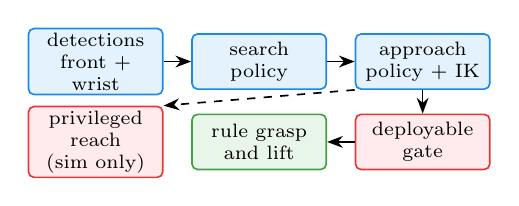
\begin{tikzpicture}[node distance=3mm and 3.5mm, font=\scriptsize,
  box/.style={draw, rounded corners=2pt, align=center, minimum height=7mm, text width=16mm, inner sep=1.5pt, line width=0.6pt},
  ar/.style={-{Stealth[length=2mm]}, line width=0.6pt}]
\node[box, fill=simF, draw=simS] (det) {detections\\front + wrist};
\node[box, fill=simF, draw=simS, right=of det] (srch) {search\\policy};
\node[box, fill=simF, draw=simS, right=of srch] (app) {approach\\policy + IK};
\node[box, fill=hwF, draw=hwS, below=of app] (gate) {deployable\\gate};
\node[box, fill=okF, draw=okS, left=of gate] (rule) {rule grasp\\and lift};
\node[box, fill=hwF, draw=hwS, left=of rule] (priv) {privileged\\reach (sim only)};
\draw[ar] (det) -- (srch);
\draw[ar] (srch) -- (app);
\draw[ar] (app) -- (gate);
\draw[ar] (gate) -- (rule);
\draw[ar, dashed] (app.south west) -- (priv.north east);
\end{tikzpicture}
\caption{Staged pipeline of Project 2. The approach ends in a gate that only uses quantities measurable on the robot;
the rule grasp starts only after that gate holds. The privileged reach criterion (dashed) is a monitor that needs the
simulator's true cube position.}
\label{fig:pipeline}
\end{figure}

% =====================================================================
\section{Method}\label{sec:method}
\subsection{Earlier stage (June 2026): teacher and students}
A state-only teacher is trained with distributional C51-SAC on a 43-D privileged observation (joint positions and
velocities, commanded targets, distance to the rest pose, cube position and orientation, tool-centre point and
tool-to-cube vector, grasp flag). The action is a 7-D delta on the commanded joint target, 0.05\,rad per step, with
hard joint limits and an elbow gate enforced inside the action term, at 10\,Hz with episodes of 10\,s. The critic has
101 atoms on $[-20, 20]$ and an ensemble of 2; the discount is 0.9. Success requires the cube to be at least 1\,mm
above its rest height, both fingers in contact and the commanded arm within 0.2\,rad of the rest pose.
A camera-based student (two 128$\times$128 RGB images and 21-D proprioception) is trained with DAgger: the frozen teacher
labels every visited state, and the probability that the teacher drives an environment is annealed from 1 to 0 over
150,000 steps. An Isaac-free deploy loop rebuilds the observation and the action limits outside the simulator.

\subsection{Project 2 (July--August 2026): staged C51-SAC on detections}
The policy is split into stages with their own actor and critic: \emph{search} until the cube is seen and centred in
the wrist camera, then, after a hand-over, \emph{approach} toward the cube (Fig.~\ref{fig:pipeline}). The search policy of training run
8951 was trained first and then frozen; the approach policy was trained in run 8953 with the search policy loaded.
Training used 256 parallel environments, 128 gradient updates per iteration, batch 512, discount 0.97 and a critic support
of $[-20, 400]$ (README, Pipeline). A spawn curriculum over a 10$\times$10 cell grid re-weights the cube spawn toward
failing cells after deterministic self-evaluation sweeps.

\textbf{Rewards.} The approach reward combines shaping terms on the wrist-image centring of the cube, its area fraction,
the jaw-mouth height above the table, hovering and table penalties, and bonuses for the success gates; the weights are
environment knobs recorded in \code{configs/project2_train_9t_dacq_2026-08-02.env}. The June reward follows the Squint
lift task.

\subsection{Success criteria}\label{sec:criteria}
\begin{itemize}
\item \textbf{search}: the episode reached the approach phase, i.e.\ the search policy handed over a cube that is seen and
  centred in the wrist camera.
\item \textbf{privileged reach}: the true 3-D distance from the jaw mouth to the cube is below 0.07\,m, held 1 frame in
  the benches. It needs the simulator's true cube position and cannot be checked on the robot.
\item \textbf{deployable gate}: the cube is centred in the wrist image (\code{APP_CEN} 0.15), the jaw mouth is low
  enough (\code{APP_MZ} 0.07\,m) and the cube's area fraction is large enough (\code{FRAC_GRASP} 0.23), all measurable
  on the robot (\code{configs/project2_bench_2026-08-03.env}).
\end{itemize}

% =====================================================================
\section{Experiments}\label{sec:experiments}
\textbf{June.} The teacher and students were trained in S1; the shipped checkpoints are in
\code{results/checkpoints/}. No training log or evaluation file of the original runs survived, so no June success rate
is reported here; the rates written in commit messages are listed as unsupported in \code{docs/claims.md}.

\textbf{Benches (2 to 3 August 2026).} A daemon benched every new approach checkpoint of run
\code{det_TP304_refac_smoke9t} together with the latest search checkpoint on a fixed eval-set grid (90 cells, later 86),
deterministically, with 32 environments and without domain randomisation: 120 benches from 128k to 3,712k
environment steps, written to \code{results/project2/bench_daemon.log}.

\textbf{Sweeps.} The training dashboards posted 114 curriculum self-evaluation sweeps of runs 8951 and 8953
(\code{ntfy_poller.log}). The sweeps used the privileged criterion, with a distance threshold between 0.07 and 0.14\,m
depending on the run's configuration file; the log has times but no dates.

\textbf{Seeded re-evaluation (2 November 2026).} The checkpoint pair of the last bench was re-evaluated with seed 0 in
S4 through the trainer's own benchmark mode, with opt-in per-episode output
(\code{scripts/eval/project2_eval.sh}): (A) a replica of the 86-cell bench, 160 episodes with cases revisited; (B) the
400-case grid, one episode per case; (C) an experimental end-to-end run with the grasp and lift rule switched on and the
episodes not ended at the reach, 86 episodes. Each run has an \code{episodes.csv} with one row per episode.

% =====================================================================
\section{Results}\label{sec:results}
\begin{table*}[t]
\centering
\caption{Project 2 in simulation (S4). Rates over eval cells (benches, sweeps) or episodes (re-evaluation, with
Wilson 95\,\% intervals). Sources: \protect\code{results/project2/}, \protect\code{docs/claims.md}.}
\label{tab:results}
\setlength{\tabcolsep}{5pt}
\begin{tabular}{@{}lccc@{}}
\toprule
 & search & privileged reach & deployable gate \\
\midrule
120 benches (Aug.) & 92.1--99.4\,\% & 84.0--95.2\,\% & \textbf{0.0\,\%} in all \\
bench of shipped pair, 86 cells & 97.8\,\% & 89.9\,\% & \textbf{0.0\,\%} \\
\midrule
A: 86-cell replica, 160 ep. & 99.4\,\% (96.5--99.9) & 88.1\,\% (82.2--92.3) & \textbf{0.0\,\%} (0.0--2.3) \\
B: 400 cases, 400 ep. & 98.5\,\% (96.8--99.3) & 73.0\,\% (68.5--77.1) & \textbf{0.0\,\%} (0.0--0.9) \\
C: end-to-end, 86 ep. & 97.7\,\% (91.9--99.4) & not measured & \textbf{0.0\,\%} (0.0--4.3) \\
\bottomrule
\end{tabular}
\end{table*}

Table~\ref{tab:results} collects the simulation results. The search stage works: 92.1--99.4\,\% of cells over the 120
benches, and 99.4\,\% (159 of 160 episodes) and 98.5\,\% (394 of 400) in re-evaluation runs A and B. The approach
reaches the cube by the privileged criterion in 84.0--95.2\,\% of cells over the benches and in 88.1\,\% (141 of 160)
and 73.0\,\% (292 of 400) of the re-evaluation episodes. Run A reproduces the logged bench of the same checkpoints
(97.8\,\%, 89.9\,\%, 0.0\,\%) within its intervals. The curriculum sweeps agree: 95--100\,\% search over 61 sweeps of run
8951, and 71--81\,\% under the privileged gate over 36 sweeps of run 8953, with a maximum of 81\,\% at 1,101k steps.

The deployable gate was never met: 0.0\,\% in all 120 benches and 0 of 646 episodes of the re-evaluation. Run C, which
switches the grasp and lift rule on, measured lift 0.0\,\% (Wilson 0.0--4.3\,\%) over 86 episodes, but it cannot test
grasping: the rule starts only after the deployable gate holds, so the grasp and lift rule itself was never exercised.

\begin{figure}[t]
\centering
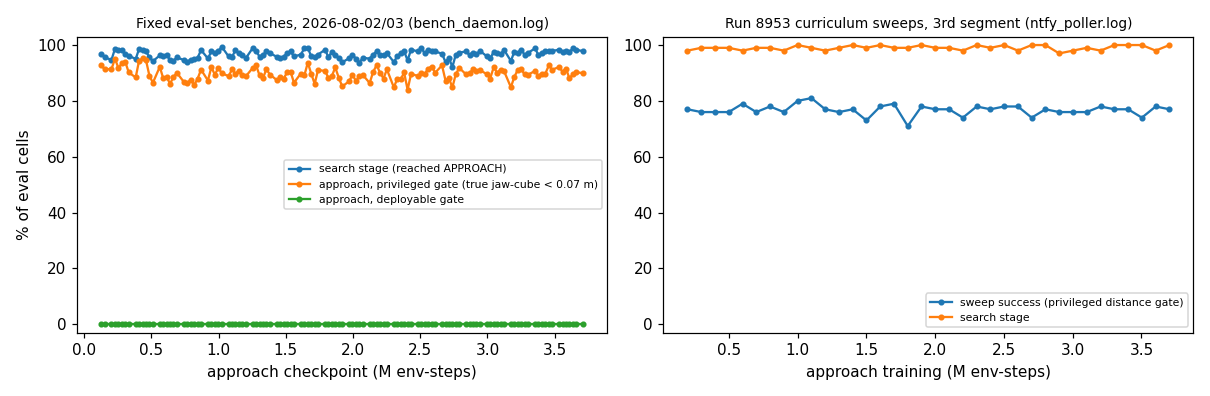
\includegraphics[width=\columnwidth]{figures/fig_log_curves.png}
\caption{Left: 120 fixed eval-set benches of successive approach checkpoints (2 to 3 August 2026); search and
privileged reach are high, the deployable gate stays at 0.0\,\% in every bench. Right: curriculum sweeps of run 8953
under its privileged gate. Rebuilt from the raw logs by \protect\code{analysis/parse_logs.py}.}
\label{fig:curves}
\end{figure}

\begin{figure}[t]
\centering
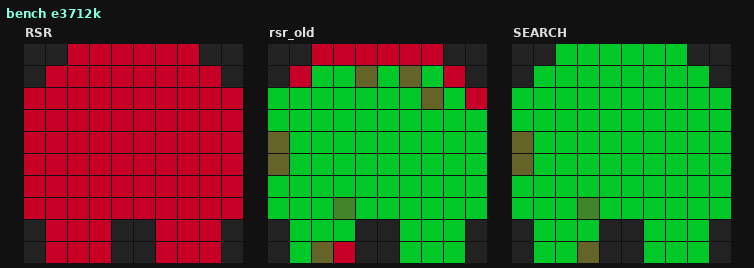
\includegraphics[width=\columnwidth]{figures/fig_bench_heatmap.png}
\caption{Per-cell results of the bench of the shipped checkpoints (3 August 2026): deployable gate (all cells failed),
privileged reach, search. Grid: lateral position $\times$ forward distance, far cells at the top; dark cells were not
evaluated.}
\label{fig:heatmap}
\end{figure}

\begin{figure}[t]
\centering
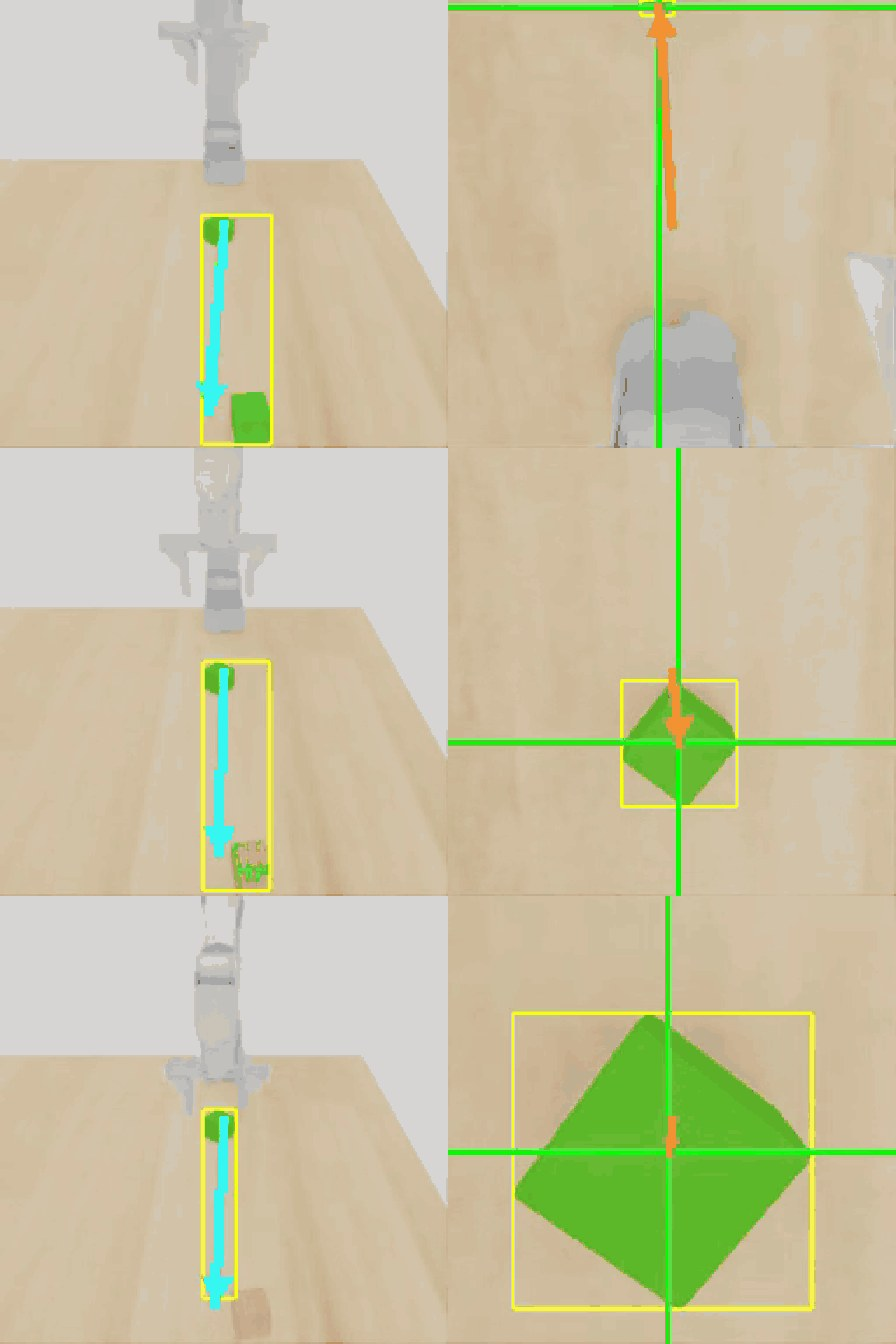
\includegraphics[width=0.55\columnwidth]{figures/fig_s4_rollout_frames.jpg}
\caption{Simulation S4, not the real robot: three frames of the first rendered episode of the shipped checkpoints
(seed 0). Left: front camera; right: wrist camera, both the detector-input views with the detection box and the arrows
drawn by the trainer. Top: search; middle: the cube centred in the wrist camera after the hand-over; bottom: the
approach close to the cube. The episode ends by the privileged criterion; the deployable gate was not met in any of
the 4 rendered episodes.}
\label{fig:rollout}
\end{figure}

% =====================================================================
\section{Hardware}\label{sec:hw}
\textbf{RL on the robot failed.} In June the camera-based DAgger student was run on the real arm and did not work: its
actions collapsed or saturated. The recorded causes are an out-of-distribution camera input (16:9 frames squashed to a
square, glare, a different background), a wrist-camera view that differed from simulation and a start pose that did
not match the simulated rest pose (Fig.~\ref{fig:inputs}). In July a residual SAC on top of a rule reach failed at its
run gate: the arm rose instead of descending, because the observations were out of distribution and the residual
accumulated until the joint limits. No Project 2 policy was run on the robot.

\textbf{The rule controller.} A separate controller was built on the robot in July: a perception thread (cube detection
on the front and wrist cameras, with open-vocabulary detection), a robot I/O thread, forward and inverse kinematics, and
a state machine with approach, follow, align, automatic grasp and lift states, plus calibration tools for the camera
intrinsics and extrinsics, the wrist camera and the gripper. The author's notes record a full pick (reach, grasp, lift)
on 7 July, grasp and lift after a forward-kinematics height correction on 13 to 14 July, and an automatic grasp cycle on
a cube at an arbitrary angle on 23 July; the same day, RL was removed from that code base. There are no trial counts,
no success rate and no video, and a repeatability sweep is listed as open. The code is kept as a record in
\code{archive/real_robot_july/}; it does not run on its own, because files with lines by a colleague (the IK engine
among them) are excluded.

\begin{figure}[t]
\centering
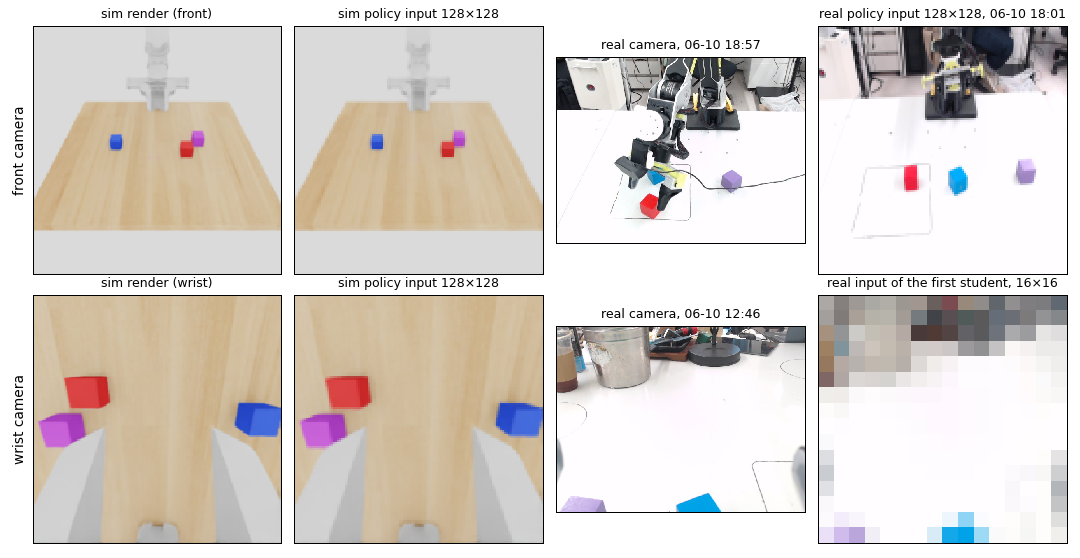
\includegraphics[width=\columnwidth]{figures/fig_student_inputs.png}
\caption{June stage. Top: front camera; bottom: wrist camera. Columns: simulated render, simulated policy input, real
camera frame, real policy input (real frames saved during real-robot diagnosis on 10 June 2026). The real wrist
camera looked over a cluttered bench instead of down between the jaws: the observation mismatch the real-robot attempt
ran into.}
\label{fig:inputs}
\end{figure}

% =====================================================================
\section{Failure analysis: why the deployable gate stayed at 0\,\%}\label{sec:failure}
The privileged criterion and the deployable gate were measured on the same episodes, so the gap is a property of the
policy, not of the evaluation. What the repository records about the cause:
\begin{itemize}
\item \textbf{Selection and curriculum used the privileged criterion.} All training entrypoints evaluated their sweeps
  with the privileged gate (\code{EVAL_SUCC_BY_OLD=1}), and the curriculum re-weighted the spawn toward cells that failed
  that criterion. The deployable gate entered training only through reward shaping and a success bonus, so the
  checkpoints were optimised and selected for a criterion the robot cannot check.
\item \textbf{The gates measure different things.} The privileged criterion is a 3-D distance below 0.07\,m. The
  deployable gate additionally requires the cube to fill a large part of the wrist image and to be centred while the
  jaw mouth is low; a gripper can be within 0.07\,m of the cube without satisfying the image conditions.
\item \textbf{Consequence for grasping.} Because the rule grasp is triggered by the deployable gate, the policy never
  reached a state from which the grasp would start; grasp and lift were never exercised in any logged run (run C).
\end{itemize}
Which of the three image conditions fails most often was not logged per episode; the re-evaluation CSVs record only the
combined gate, so this report does not rank them.

% =====================================================================
\section{Limitations}\label{sec:limits}
\begin{itemize}
\item No RL policy was shown working on the hardware; moving a learned policy to the robot did not succeed in
  either stage. The hardware results come from the rule controller and are uncounted notes.
\item In simulation the deployable gate was 0.0\,\% in all 120 benches; the high rates use the search criterion or a
  privileged distance. There is no end-to-end grasp and lift success in simulation.
\item The August numbers come from aggregate logs (per bench or per sweep); only the re-evaluation of 2 November has
  per-episode files. The sweep log carries no dates, and its threshold is not printed per sweep.
\item Not reproducible end to end from the repository alone: Isaac Sim, Isaac Lab, the LeIsaac fork with the reBot
  configuration, the robot assets and the YOLO-OBB detector weights are not included.
\end{itemize}

% =====================================================================
\section{Reproducibility}\label{sec:repro}
\textbf{Layout} (after the restructure of 5 November 2026, \code{docs/refactor_2026-11.md}):
\code{src/rebot_grasp_rl/} (Project 2 trainer, networks, evaluation hooks), \code{src/rebot_grasp_env/} (S4
environment), \code{src/rebot_teacher_student/} (June stage and the Isaac-free deploy loops),
\code{scripts/} (launchers), \code{configs/}, \code{results/} (logs, re-evaluation CSVs, checkpoints),
\code{analysis/} (checkers), \code{archive/} (records). The restructure was checked to be a pure move and rename of
the previous code.

\textbf{Without Isaac Sim} one can install the package, run the tests, rebuild the logged numbers
(\code{python analysis/parse_logs.py --check}), recompute the re-evaluation rates and intervals from the CSVs
(\code{python analysis/project2_eval_summary.py results/project2/reeval/bench86}), run the June deploy loops against
mock robots (\code{bash scripts/deploy/mock_deploy.sh}), and check every number of the README and of this report
(\code{python analysis/verify_claims.py}, \code{python analysis/verify_report.py}).

\textbf{With Isaac Sim} (Isaac Sim 5.1, Isaac Lab 2.3, the LeIsaac reBot fork, detector weights): training and the
re-evaluation, \code{OUT=<dir> bash scripts/eval/project2_eval.sh A B C}.

\textbf{Attribution.} All code in the repository is the author's. The teacher, the students and the Project 2 trainer
follow Squint's design~\cite{squint} and share only generic lines with it; its MIT notice is included. LeIsaac, Isaac
Lab and Ultralytics are used as installed libraries; the vendor robot assets are not redistributed
(\code{docs/third_party.md}).

% =====================================================================
\section{Conclusion}\label{sec:conclusion}
A staged C51-SAC on detection-level observations learned to search for the cube and to approach it in simulation, but
only by a criterion that needs the simulator's true cube position: the gate a robot could check was met in no bench and
in 0 of 646 re-evaluation episodes, so the rule grasp never started. Moving learned policies to the reBot failed in both
recorded attempts, while a perception, kinematics and state-machine controller is recorded as grasping and lifting the
cube without counted trials. The clearest lesson is to optimise, select and report against the deployable criterion
from the start; the next step is to log the gate's components per episode and train with the deployable gate as the
sweep and selection criterion.

\begin{thebibliography}{99}
\bibitem{haarnoja2018sac} T.~Haarnoja, A.~Zhou, P.~Abbeel, and S.~Levine, ``Soft actor-critic: Off-policy maximum
entropy deep reinforcement learning with a stochastic actor,'' in \emph{Proc. ICML}, 2018.
\bibitem{bellemare2017c51} M.~G.~Bellemare, W.~Dabney, and R.~Munos, ``A distributional perspective on reinforcement
learning,'' in \emph{Proc. ICML}, 2017.
\bibitem{squint} A.~Almuzairee, ``Squint,'' GitHub repository \url{https://github.com/aalmuzairee/squint}, MIT License, 2026.
\bibitem{chen2019lbc} D.~Chen, B.~Zhou, V.~Koltun, and P.~Kr\"ahenb\"uhl, ``Learning by cheating,'' in \emph{Proc. CoRL},
2019.
\bibitem{ross2011dagger} S.~Ross, G.~Gordon, and D.~Bagnell, ``A reduction of imitation learning and structured prediction
to no-regret online learning,'' in \emph{Proc. AISTATS}, 2011.
\bibitem{pinto2018asymmetric} L.~Pinto, M.~Andrychowicz, P.~Welinder, W.~Zaremba, and P.~Abbeel, ``Asymmetric actor
critic for image-based robot learning,'' in \emph{Proc. RSS}, 2018.
\bibitem{tobin2017dr} J.~Tobin, R.~Fong, A.~Ray, J.~Schneider, W.~Zaremba, and P.~Abbeel, ``Domain randomization for
transferring deep neural networks from simulation to the real world,'' in \emph{Proc. IROS}, 2017.
\bibitem{mittal2023orbit} M.~Mittal \emph{et al.}, ``Orbit: A unified simulation framework for interactive robot learning
environments,'' \emph{IEEE Robotics and Automation Letters}, 2023.
\bibitem{leisaac} LightwheelAI, ``LeIsaac,'' GitHub repository \url{https://github.com/LightwheelAI/leisaac}, Apache-2.0.
\bibitem{ultralytics} G.~Jocher \emph{et al.}, ``Ultralytics YOLO,'' software, \url{https://github.com/ultralytics/ultralytics}, AGPL-3.0.
\bibitem{minderer2023owlv2} M.~Minderer, A.~Gritsenko, and N.~Houlsby, ``Scaling open-vocabulary object detection,'' in
\emph{Proc. NeurIPS}, 2023.
\bibitem{buss2004ik} S.~R.~Buss, ``Introduction to inverse kinematics with Jacobian transpose, pseudoinverse and damped
least squares methods,'' technical report, University of California, San Diego, 2004.
\bibitem{wilson1927} E.~B.~Wilson, ``Probable inference, the law of succession, and statistical inference,''
\emph{Journal of the American Statistical Association}, 1927.
\end{thebibliography}
\end{document}
